\documentclass{article}%
\usepackage[T1]{fontenc}%
\usepackage[utf8]{inputenc}%
\usepackage{lmodern}%
\usepackage{textcomp}%
\usepackage{lastpage}%
\usepackage[head=40pt,margin=0.5in,bottom=0.6in]{geometry}%
\usepackage{graphicx}%
%
\title{\textbf{ONG denunciaron las detenciones arbitrarias en Venezuela ante la CIDH}}%
\author{El Nacional Web}%
\date{05/12/2018}%
%
\begin{document}%
\normalsize%
\maketitle%
\textbf{URL: }%
http://www.el{-}nacional.com/noticias/politica/ong{-}denunciaron{-}las{-}detenciones{-}arbitrarias{-}venezuela{-}ante{-}cidh\_262245\newline%
%
\textbf{Periodico: }%
EN, %
ID: %
262245, %
Seccion: %
Política\newline%
%
\textbf{Palabras Claves: }%
Política, Presos políticos\newline%
%
\textbf{Derecho: }%
18%
, Otros Derechos: %
5, 12%
, Sub Derechos: %
12.1.3%
\newline%
%
\textbf{EP: }%
NO\newline%
\newline%
%
\textbf{\textit{Varios entes denunciaron que los procesos judiciales de los presos políticos conllevan a la violación de los derechos humanos~}}%
\newline%
\newline%
%
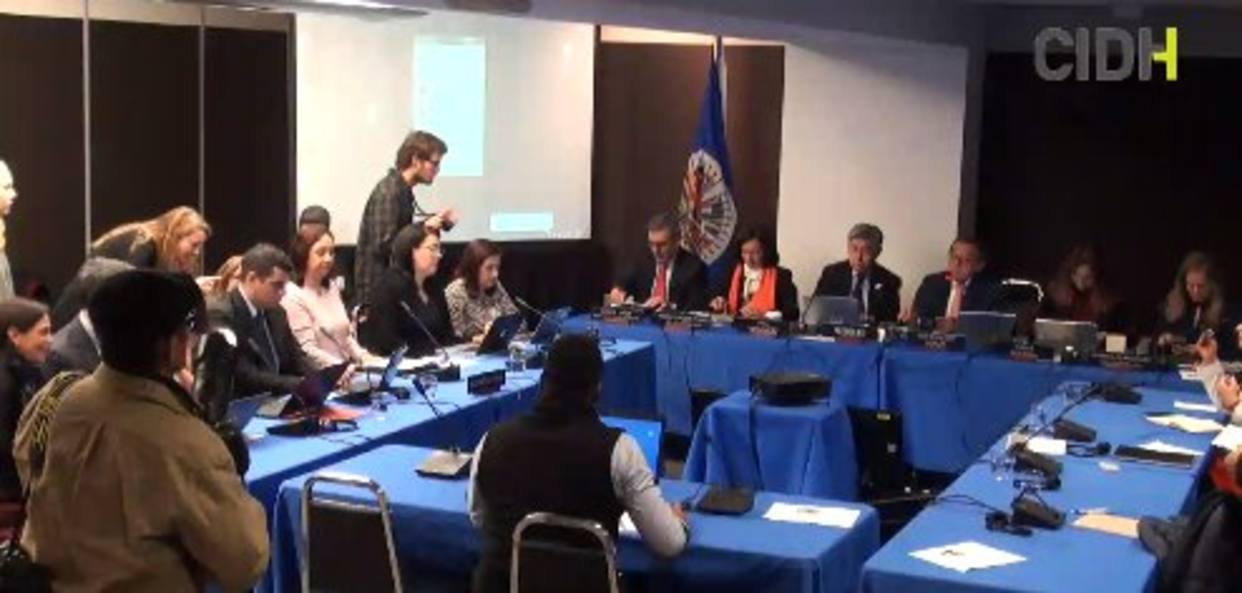
\includegraphics[width=300px]{27.jpg}%
\newline%
%
Varias organizaciones no gubernamentales denunciaron este miércoles ante la Comisión Interamericana de los Derechos Humanos (CIDH) que los procesos judiciales de los presos políticos y las detenciones arbitrarias son demostraciones de violación de derechos humanos en Venezuela.%
\newline%
%
Edison Lanza, relator especial para la libertad de expresión de la CIDH, destacó el caso de los dos bomberos aprehendidos por hacer un video de sátira por demostrar la subjetividad de las autoridades judiciales.%
\newline%
%
“El gobierno percibe como lo contrario a sus fines lo reprime, lo hace a través de la detención y la eliminación de garantías. Si no se realizan acciones que contribuyan a desarmar esta estructura, es difícil que las audiencias tengan algún tipo de repercusión”, resaltó Lanza.%
\newline%
%
Foro Penal indicó ante la comisión que se registraron 13.000 detenciones arbitrarias desde 2014 hasta la fecha y que existen 288 presos políticos en el país, y que en ellas se cuentan a los 59 colombianos retenidos en La Yaguara desde septiembre de 2016, quierenes fueron tildados como paramilitares por el presidente Nicolás Maduro.%
\newline%
%
“A través del uso del sistema judicial, el gobierno venezolano viola los derechos humanos, mantiene privadas de libertad a las personas arbitrariamente y vulnera el derecho a la salud, la integradid física y psicológica y no cumple con el debido proceso de defensa”, sentenció el representante de la ONG.%
\newline%
%
La organización AC Sinergia denunció el caso de Rubén González, sindicalista de Ferrominera,~ante la CIDH, alegando que su detención fue realizada ante tribunales militares. “Se violó su derecho a la libertad de expresión, libertad sindical, derecho al trabajo y a la defensa de los trabajadores. Queremos relevar las condiciones restrictivas recientes de violación de derechos humanos a este gremio”, aseveró la delegada de la organización.%
\newline%
%
Otras ONG resaltaron la vulneración al derecho de ejercicio político, presentando una disminución de los mismos en 90\% en el país. Además, los ataques a los dirigentes políticos se ha agudizado, violando sus derechos.%
\newline%
%
“Al menos ocho~diputados a la Asamblea Nacional están fuera del país por persecución, cuatro de ellos~han sido presos y torturados. Tres parlamentarios~han sido suspendidos de sus cargos, a seis legisladores~les anularon los pasaportes y tres diputados~han sido inhabilitados en al menos 75 sentencias del Tribunal Supremo de Justicia”, indicó Transparencia Venezuela.%
\newline%
%
\end{document}